\documentclass{beamer}
\usetheme{CambridgeUS}
\usecolortheme{beaver}
\usepackage[utf8]{inputenc}
\usepackage[T1]{fontenc}
\usepackage{amsmath,amssymb,amsthm}
\usepackage{mathrsfs}
\usepackage{geometry}
\usepackage{graphicx}
\usepackage{xcolor}            % load xcolour before hyperref
\usepackage{tikz}
\usetikzlibrary{
  arrows.meta,
  patterns,
  positioning,
  decorations.pathmorphing,
  calc
}
\usepackage{tcolorbox}
\usepackage{float}
\setbeamertemplate{navigation symbols}{}


\title{The Wasserstein Distance}
\author{Alex Cristaudo}
\institute[UCT]{University of Cape Town}
\date{27 October 2025}
\setbeamerfont{footline}{size=\tiny}

\begin{document}

% TITLE SLIDE
\begin{frame}
  \titlepage
\end{frame}


% INTRODUCTION
\begin{frame}{Introduction}
  \textbf{What is the Wasserstein distance?}
  \begin{itemize}
    \item A metric between probability measures.
    \item Gives the minimal cost for transforming one probability measure into another.
    \item The concept of optimal transport originated by Monge (1781); refined by Kantorovich in 1940s. We consider Kantorovich's formulation.
  \end{itemize}

  \textbf{Key Question}:
  \begin{quote}
    Given two distributions of mass, what is the optimal way (in terms of a \emph{cost}) to transform one mass into the other?
  \end{quote}
\end{frame}

% OPTIMAL TRANSPORT INTUITION
\begin{frame}{Optimal Transport: Intuition}
      \textbf{Intuitive scenario:} Suppose we have defined the following:
      \begin{itemize}
        \item Move a pile of mass $X$ into a hole $Y$ so all mass matches. Assume both have a mass of one.
        \item Distributions $\mu$, $\nu$ represent mass at $X$ and $Y$. 
        \item Cost function $c(x, y)$ quantifies the expense of moving a unit mass from $x$ to $y$.
        \item Transport plan $\gamma(x, y)$: how much mass is transported from $x$ to $y$.
      \end{itemize}
      \begin{center}
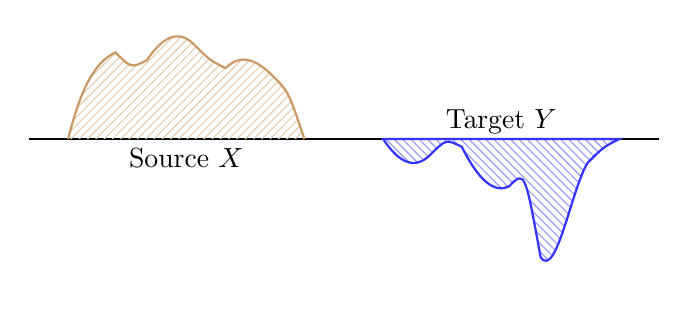
\begin{tikzpicture}[scale=1]

% Ground line
\draw[thick] (-4,-0.5) -- (4,-0.5);

% More complex pile of mass (source distribution μ) - multi-peaked
\fill[brown!60, pattern=north east lines, pattern color=brown!40] 
    (-3.5,-0.5) .. controls (-3.3,0.3) and (-3.1,0.5) .. (-2.9,0.6) 
    .. controls (-2.7,0.4) .. (-2.5,0.5) 
    .. controls (-2.3,0.8) and (-2.1,0.9) .. (-1.9,0.7)
    .. controls (-1.7,0.5) .. (-1.5,0.4)
    .. controls (-1.3,0.6) and (-1.1,0.5) .. (-0.9,0.3)
    .. controls (-0.7,0.1) .. (-0.5,-0.5) -- cycle;

\draw[thick, brown!80] 
    (-3.5,-0.5) .. controls (-3.3,0.3) and (-3.1,0.5) .. (-2.9,0.6) 
    .. controls (-2.7,0.4) .. (-2.5,0.5) 
    .. controls (-2.3,0.8) and (-2.1,0.9) .. (-1.9,0.7)
    .. controls (-1.7,0.5) .. (-1.5,0.4)
    .. controls (-1.3,0.6) and (-1.1,0.5) .. (-0.9,0.3)
    .. controls (-0.7,0.1) .. (-0.5,-0.5);

% More complex hole (target distribution ν) - multi-depression with same total area
\fill[blue!60, pattern=north west lines, pattern color = blue!40] 
    (0.5,-0.5) .. controls (0.7,-0.8) and (0.9,-0.9) .. (1.1,-0.7)
    .. controls (1.3,-0.5) .. (1.5,-0.6)
    .. controls (1.7,-1.0) and (1.9,-1.2) .. (2.1,-1.1)
    .. controls (2.3,-0.9) .. (2.5,-2.0)
    .. controls (2.7,-2.3) and (2.9,-1.1) .. (3.1,-0.8)
    .. controls (3.3,-0.6) .. (3.5,-0.5) -- cycle;

\draw[thick, blue!80] 
    (0.5,-0.5) .. controls (0.7,-0.8) and (0.9,-0.9) .. (1.1,-0.7)
    .. controls (1.3,-0.5) .. (1.5,-0.6)
    .. controls (1.7,-1.0) and (1.9,-1.2) .. (2.1,-1.1)
    .. controls (2.3,-0.9) .. (2.5,-2.0)
    .. controls (2.7,-2.3) and (2.9,-1.1) .. (3.1,-0.8)
    .. controls (3.3,-0.6) .. (3.5,-0.5) -- cycle;

% Labels
\node[below] at (-2,-0.5) {Source $X$};
\node[below] at (2,0) {Target $Y$};

\end{tikzpicture}
\end{center}
\end{frame}


\begin{frame}{Optimal Transport: Intuition}
We must have the following:
\begin{enumerate}
    \item The amount we move out of $x$ is the same as the amount it started with. That is, \[
    \int_Y \gamma (x,y) dy = \mu (x)
    \]
    \item The amount moved into point $y$ must equal the depth of the hole. That is, \[
    \int_X \gamma (x,y) dx = \nu (y)
    \]
\end{enumerate}
which is to say
\[
\int _Y \int _X \gamma (x,y) dydx = \int_X \mu (x) dx = \int_Y \nu (y) dy
\]
This is equivalent to the requirement that $\gamma$ is a joint probability distribution with marginals $\mu$ and $\nu$. 
\end{frame}

\begin{frame}{Optimal Transport: Intuition}
The total cost of a transport plan $\gamma$ is \[
\int _Y \int _X c(x,y) \gamma (x,y) dxdy
\]
The plan $\gamma$ is not unique. Any probability distribution with marginals $\mu$ and $\nu$ represents a viable transport plan. We want the optimal transport plan to be the one with the minimum total cost. \\ \textbf{NOTE:} We will instead use probability measures, as a generalisation of probability distributions, allowing for varied mass distributions.

    \begin{figure}[h]
        \begin{center}
        \includegraphics[scale = 0.2]{transport.png}
\end{center}
    \end{figure}
\end{frame}

% MATHEMATICAL FOUNDATIONS
\begin{frame}{Mathematical Foundations: The Kantorovich Problem}
  \textbf{Suppose we have the following}
  \begin{itemize}
    \item $(X, d_X)$, $(Y, d_Y)$: Polish metric spaces (complete separable metric spaces)
    \item $(X, \mathcal{F}_1), (Y, \mathcal{F}_2)$: measurable spaces
    \item $\mathcal{P}(X) :=$ the set of probability measures on $(X, \mathcal{F}_1)$\\ $\mathcal{P}(Y) :=$ the set of probability measures on $(Y, \mathcal{F}_2)$\\ $\mathcal{P}(X \times Y) :=$ the set of probability measures on $(X \times Y, \mathcal{F}_1 \otimes \mathcal{F}_2)$.
    \item $c(x, y)$: cost function (= a nonnegative $\mathcal{F}_1 \otimes \mathcal{F}_2$-measurable function)
  \end{itemize}
~\\ For $\mu \in \mathcal{P}(X), \nu \in \mathcal{P}(Y)$, we define the set of \textbf{Transport Plans} as:
  \small{\[
  \Pi(\mu,\nu) = \{\gamma \in \mathcal{P}(X \times Y) : \forall A_i \in \mathcal{F}_i, \gamma (A_1 \times Y) = \mu (A_1), \gamma (X \times A_2) = \nu (A_2)\}
  \]}
  \normalsize The Kantorovich Problem is to find $\gamma$ that attains the infimum:
  \[
    \mathcal{K}(\mu, \nu) = \inf_{\gamma \in \Pi(\mu, \nu)} \int_{X \times Y} c(x, y) d\gamma(x, y)
  \]
  Such a transport plan always exists.
\end{frame}

% THE WASSERSTEIN DISTANCE
\begin{frame}{The Wasserstein Distance}
  Let $p \ge 1$. The $p$-Wasserstein Distance is a special case of the Kantorovich Problem, where:
  \begin{itemize}
    \item We only consider one Polish metric space $(X,d)$
    \item The cost function is $c(x,y) = d(x,y)^p$
    \item The measurable space is $(X, \mathcal{B}(X))$ where $\mathcal{B}(X)$ is the Borel $\sigma$-algebra on $X$.
  \end{itemize}

  \begin{block}{Definition (Finite $p$-th moment)}
  Fix $x_0 \in X$. A measure $\mu \in \mathcal{P}(X)$ is said to have finite $p$-th moment if \[
\int _X d(x,x_0)^p d\mu (x) < \infty\]
  \end{block}

  We restrict our space of measures to be the set of measures that have finite $p$-th moment (denoted $\mathcal{P}_p(X)$)
\end{frame}

\begin{frame}{The Wasserstein Distance}
  Now we are ready to define the $p$-Wasserstein Distance
  \begin{block}{Definition (p-Wasserstein Distance)}
    For $p \geq 1$ and $\mu, \nu \in \mathcal{P}_p(X)$, the $p$-Wasserstein distance is:
    \[
      \mathcal{W}_p(\mu, \nu) = \left(\inf_{\gamma \in \Pi(\mu, \nu)} \int_{X \times X} d(x, y)^p d\gamma(x, y)\right)^{1/p}
    \]
    We then define \[
    \mathcal{W}_\infty (\mu, \nu) := \lim \limits _{p \to \infty} \mathcal{W}_p (\mu, \nu)
    \]
  \end{block}
\end{frame}

% KEY THEOREMS
\begin{frame}{Key Theorems and Remarks}
  \begin{itemize}
    \item \textbf{Existence:} For $\mu, \nu \in \mathcal{P}_p(X)$, an optimal plan $\gamma^\ast$ attains the infimum.
    \item \textbf{Metric Properties:} $\mathcal{W}_p$ defines a metric.
    \item \textbf{Completeness:} If $(X, d)$ is complete, $(\mathcal{P}_p, \mathcal{W}_p)$ is complete. 
%     \item \textbf{Usage:} The most commonly used variants are:
% \begin{itemize}
% \item \( \mathcal{W}_1 \): The 1-Wasserstein distance (the Earth Mover's Distance). This tries to minimise the total effort which is directly propertional to mass and distance 
% \item \( \mathcal{W}_2 \): The 2-Wasserstein distance. This is proportional to $\sqrt{\text{mass} \times \text{distance}^2}$ and penalises large movements more.
% \item \( \mathcal{W}_\infty \): The infinity Wasserstein distance. This represents the worst-case transport distance (the farthest any mass particle moves). Mass does not matter, only the maximum distance.
% \end{itemize}
  \end{itemize}
\end{frame}

% KANTOROVICH-RUBINSTEIN DUALITY
\begin{frame}{Kantorovich-Rubinstein Duality}
  One of the most important results in optimal transport theory is the Kantorovich-Rubinstein duality theorem, which provides an equivalent characterization of the 1-Wasserstein distance.
  \begin{block}{The Kantorovich-Rubinstein Duality}
    For $\mu, \nu \in \mathcal{P}_1(X)$ on a complete separable metric space $(X, d)$:
    \[
      \mathcal{W}_1(\mu, \nu) = \sup\left\{\int_X f d\mu - \int_X f d\nu : f : X \to \mathbb{R} \text{ is 1-Lipschitz}\right\}
    \]
  \end{block}
  This duality allows us to check Lipschitz maps instead of all possible couplings.
\end{frame}

\begin{frame}{Example: Dirac Measures}
For $a,b,c \in \mathbb{R}$, \begin{itemize}
  \item $\mu = \frac{1}{2} \delta_a + \frac{1}{2} \delta _b$
  \item $\nu = \delta _c$
\end{itemize}
By using 1-Lipschitz maps, we can easily show \[\mathcal{W}_1(\mu, \nu) = \frac{1}{2} |a-c| + \frac{1}{2} |b-c|\]
\end{frame}

% EXAMPLES
\begin{frame}{Real Probability Measures}
  Consider measures \( \mu \) and \( \nu \) on \( \mathbb{R} \) with associated CDFs \( F \) and \( G \). So \begin{align*}F(x) &= \mu ((-\infty, x]) \\ G(x) &= \nu ((-\infty, x])\end{align*}
We first define the Quantile Function in terms of these CDFs:

\begin{definition}[Quantile Function]
Let \(F\colon\mathbb{R}\to[0,1]\) be a cumulative distribution function.  The \emph{quantile function} \(F^{-1}\colon[0,1]\to \overline{\mathbb{R}}\) is defined by
\[
  F^{-1}(p) = \begin{cases}\inf\{x \in \mathbb{R} : F(x) > 0\} & \text{if } p = 0 \\ \inf\{x \in \mathbb{R} : F(x) \geq p\} & \text{if } p \in (0,1]\end{cases}
\]
\end{definition}
\end{frame}

\begin{frame}{One-Dimensional Wasserstein Measures}
We can then find the $p$-Wasserstein Distance in terms of this Quantile Function:
\begin{theorem}[One-Dimensional Wasserstein] \label{thm:1d} For $\mu, \nu \in \mathcal{P}_p(\mathbb{R})$,
\[
\mathcal{W}_p(\mu,\nu) = \left(\int_0^1 |F^{-1}(t) - G^{-1}(t)|^p dt\right)^{1/p}
\]
where \( F^{-1} \) and \( G^{-1} \) are the quantile functions of $\mu$ and $\nu$ respectively.
\end{theorem}
\noindent
Intuitively, this is saying that our minimum transportation plan corresponds to moving the mass in $\mu$, corresponding to quantile $t$ in $F$ into the corresponding quantile value in $\nu$.

\end{frame}

\begin{frame}{Example: Uniform Distributions}
Consider uniform measures $\mu, \nu \in \mathcal{P}(\mathbb{R})$ defined by \begin{align*}
\mu (A) & := \lambda _1 (A \cap [0,1]) \\ 
\nu (A) & := \frac{\lambda _1 (A \cap [0,2]) }{2}
\end{align*}
For our canonical random variable $X_\mu \sim U(0,1)$ and $X_\nu \sim U(0,2)$. Then \[F(t) = tI_{[0,1)} + I_{[1,\infty]} \Longrightarrow F^{-1}(t) = t\]
\[G(t) = \frac{1}{2}tI_{[0,2)} + I_{[2,\infty]} \Longrightarrow G^{-1}(t) = 2t\]
Both clearly have finite 1 and 2-moments, so the 1-Wasserstein and 2-Wasserstein distances are:
\footnotesize
\[
\mathcal{W}_1(\mu,\nu) = \int_0^1 |t - 2t| dt = \int_0^1 t dt = \frac{1}{2}
\]
\[
\mathcal{W}_2(\mu,\nu) = \left(\int_0^1 |t - 2t|^2 dt\right)^{1/2} = \left(\int_0^1 t^2 dt\right)^{1/2} = \frac{1}{\sqrt{3}}
\]
\normalsize
\end{frame}

% MULTIVARIATE NORMALS
\begin{frame}{Example: Multivariate Normal Distributions}
  \begin{block}{Theorem}
    For $\mu = N(\mathbf{m}_1, \Sigma_1)$, $\nu = N(\mathbf{m}_2, \Sigma_2)$ on $\mathbb{R}^d$:
    \[
      \mathcal{W}_2^2(\mu, \nu) = |m_1 - m_2|^2 + \mathrm{tr}\left(\Sigma_1 + \Sigma_2 - 2 \left(\Sigma_1^{1/2}\Sigma_2\Sigma_1^{1/2}\right)^{1/2}\right)
    \]
  \end{block}
  In the univariate case, we can show, using this and the quantile functions: ~\\
  \tiny
  \begin{align*} \mathcal{W}_1(\mu, \nu) &= 
\begin{cases}
|m_1 - m_2|, & \text{if } \sigma_1 = \sigma_2, \\[10pt]
|m_1 - m_2|
\left[
2\,\Phi\!\left(
\dfrac{|m_1 - m_2|}{|\sigma_1 - \sigma_2|}
\right)
- 1
\right]
+ 
|\sigma_1 - \sigma_2|
\sqrt{\dfrac{2}{\pi}}
\exp\!\left(
-\dfrac{(m_1 - m_2)^2}{2(\sigma_1 - \sigma_2)^2}
\right),
& \text{if } \sigma_1 \neq \sigma_2,
\end{cases} \\ \\  \mathcal{W}_2 (\mu, \nu) &= \sqrt{(m_1-m_2)^2 + (\sigma_1-\sigma_2)^2}
  \end{align*}
\end{frame}

% STABILITY PROPERTIES
\begin{frame}{Stability Under Weak Convergence}
  \begin{block}{Definition: Weak Convergence}
  We say a sequence of measures $(\mu_n)_{n \in \mathbb{N}}$ converges weakly to a measure $\mu$ (denoted $\mu_n \rightharpoonup \mu$) if $X_n \sim \mu_n$ and $X \sim \mu$ implies $X_n \xrightarrow{\mathcal{D}} X$
  \end{block}
  \begin{theorem}[Stability Under Weak Convergence]
  Let a sequence $(\mu_n)_{n \in \mathbb{N}}\subseteq\mathcal{P}_p(X)$ and $\mu\in\mathcal{P}_p(X)$. Then the following are equivalent:
\begin{enumerate}
  \item $\mathcal{W}_p(\mu_n,\mu)\to0$ as $n\to\infty$.
  \item 
    \begin{enumerate}
      \item $\mu_n$ converges weakly to $\mu$ (i.e.\ $\mu_n \rightharpoonup \mu$),
      \item the $p$th moments converge. For any fixed $x_0 \in X$:
      \[
        \int_{X} d(x,x_0)^p\,d\mu_n(x)
        \to 
        \int_{X} d(x,x_0)^p\,d\mu(x)
        \quad\text{ as } n \to \infty.
      \]
    \end{enumerate}
\end{enumerate}
\end{theorem}
\textbf{Example:} If $\mu_n = N(0, \frac{1}{n})$, then $\mu _n \to \delta_0$ with respect to the $\mathcal{W}_p$ metric.
\end{frame}


% APPLICATION: COLOUR TRANSFER
\begin{frame}{Application: Colour Transfer}
  \begin{itemize}
    \item Recolouring an image with the colours from another image.
    \item Represent images as probability measures over $\mathbb{R}^3$ (using their colours - RGB).
    \item Use computational methods to approximate the optimal transport plan.
    \item The Wasserstein distance measures the minimal effort needed to transform one colour distribution into another.
    \item This not only compares which colours appear in each image, but how far apart they are in colour space. It accounts for whether colours are similar or not already.
  \end{itemize}

\end{frame}

\begin{frame}{Application: Colour Transfer}
    \begin{figure}[h]
\begin{center}
  \includegraphics[scale = 0.2]{colour_distributions.png}
\end{center}
\end{figure}

Our output image, that takes the colours in the target image and applies them to our source image, looks something like:

\begin{figure}[h]
\begin{center}
  \includegraphics[scale = 0.2]{output.png}
\end{center}
\end{figure}
\end{frame}

\begin{frame}{Questions}
\centering 
\Huge Thank You! Any Questions?
\end{frame}

\end{document}